\section{Analysis}

\begin{figure}
    \centering
    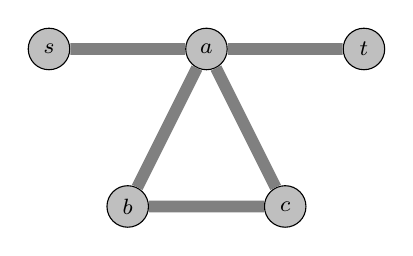
\begin{tikzpicture}
        \tikzstyle{every node}=[circle, fill=lightgray, draw=black, inner sep=2pt, minimum size=1.5em, font=\footnotesize, text=black]
        \tikzstyle{edge}=[gray, line width=1.5mm]
    
        \node (s) at (0,2) {$s$};
        \node (a) at (2,2) {$a$};
        \node (b) at (1,0) {$b$};
        \node (c) at (3,0) {$c$};
        \node (t) at (4,2) {$t$};
    
        \draw[edge] (s) -- (a) -- (b) -- (c) -- (a) -- (t);
    \end{tikzpicture}
    \caption{No odd $s$-$t$-path exist, yet we still have many odd $s$-$t$-walks.}
    \label{figure:small2}
 \end{figure}

Consider \Cref{figure:small2}. There are no odd paths from $s$ to $t$, yet we have an infinite amount of odd walks by utilizing the cycles $[a,b,c]$ or $[a,c,b]$ an odd number of times to offset the parity. Our algorithm would first find an odd walk to $a$, then an even walk to $b$, then an odd walk to $c$, then an even walk to $a$, and lastly an odd walk to $t$. However, then $a$ is used twice in the walk, once for each parity, and the resulting walk is not a path. Therefore can this algorithm not be used to solve \textsc{Shortest Odd Path}.

\subsection{Limitations}
The main limitation of the algorithm is that the edges in the input graph must have either non-negative weights or no weights at all. Otherwise we cannot guarantee that \pyth{even_dist[u]} and \pyth{odd_dist[u]} have their final, correct values when we scan a vertex $u$. 

Note that unlike most other algorithms shown in this thesis, this algorithm does not require the input graph to be undirected, it can also be directed.

\subsection{Correctness}
Let \pyth{(priority, even, u)} be the triple at the front of the queue at any point in the execution of our algorithm.
Claim: If \pyth{even} is true and \pyth{even_done[u]} is false, then \pyth{priority} is the cost of the shortest even path from the source to \pyth{u}.

\begin{proof}
By induction. 

The source vertex \pyth{s} has a best possible even cost of \pyth{0}, and initially we have only \pyth{(0, true, s)} in the queue. When that triple is popped the property holds in the base case.

\todo[inline]{
    Burde yoinke beviset herfra: https://web.engr.oregonstate.edu/~glencora/wiki/uploads/dijkstra-proof.pdf

    Eller herfra: https://community.wvu.edu/~krsubramani/courses/fa05/gaoa/qen/dijk.pdf

    Eller fra INF234

    Også si det samme når det er odd, kanskje
}

\end{proof}

\subsection{Complexity}
Let $(G,s,t)$ be an instance of \textsc{Shortest Odd Walk}, let $n := |V|$ and let $m := |E|$.\\
Claim: the algorithm runs in time at most $O(m \cdot \log m)$, or $O(m \cdot \log n)$ if the graph is simple.
\begin{proof}
    Because of our \pyth{odd_done} and \pyth{even_done} arrays, we can guarantee that each vertex is scanned at most twice, once for each parity. For each scan, we loop through each of the neighbours in linear time, and consider putting them in the queue. The total cost of the scans is therefore at most $O(m)$. A vertex may be put into the queue many times before it is scanned, in the worst case once for each of its neighbours. That means that we put vertices in the queue at most $O(m)$ times, for a total cost of $O(m)$, and removing all of them takes a total of $O(m \cdot \log m)$. 
    
    The algorithm runs in time at most $O(m) + O(m \cdot \log m) = O(m \cdot \log m)$, which shows the first part of the claim.
    
    If the graph is simple we may simplify the complexity further: $O(m \cdot \log m) \subseteq (m \cdot \log n^2) = O(m \cdot 2 \cdot \log n) = O(m \cdot \log n)$, which shows the second part of the claim.
\end{proof}

\subsection{Benchmarking}

\todo[inline]{Do the benchmarking, silly}

\subsection{Discussion}
Though we discovered it ourselves, the algorithm is not particularly groundbreaking or in any way creative. Thus, we do not expect it to be original. It is, however, quite fast, and we are happy with that. The main reason we include it in this thesis is because of its pedagogical value in introducing our main topic: \textsc{Shortest Odd Path}. \todo{Skrive mer her?}